\documentclass[aspectratio=169]{beamer} % 16:9 aspect ratio for modern screens

% Theme settings
\usetheme[progressbar=foot]{metropolis} % Minimalist theme
\metroset{progressbar=frametitle} % Progress bar soll nur folien mit titel berücksichtigen?

\makeatletter
    \setlength{\metropolis@progressinheadfoot@linewidth}{1.5pt}
\makeatother


\usefonttheme{professionalfonts} % Font theme

% Packages
\usepackage[T1]{fontenc}   % Font encoding
\usepackage[ngerman]{babel} % German language
\usepackage[sfdefault]{FiraSans} % For FiraSans font
\usepackage[backend=biber, style=authoryear-comp
, sorting=nyt]{biblatex} % For bibliography
\usepackage{csquotes} % Recommended for biblatex with babel/polyglossia
\usepackage{textgreek} % Greek letters in text mode (aus references von Citavi)
\usepackage{tikz}          % For drawing graphics

\usepackage{graphicx}       % For including images
\usepackage{amsmath, amssymb} % For math symbols

% Bibliography settings
\addbibresource{references.bib} % Path to the bibliography file

% custom Citation commands
\DeclareCiteCommand{\citeauthortitle}
  {\usebibmacro{prenote}}
  {\usebibmacro{citeindex}%
   \printnames{labelname}%
   \setunit{\space\textendash\space}% <- Hier wird das Trennzeichen ":" hinzugefügt
   \printfield{title}}
  {\multicitedelim}
  {\usebibmacro{postnote}}

\DeclareCiteCommand{\parenciteauthortitle}
  {\usebibmacro{prenote}}
  {\bibopenparen\usebibmacro{citeindex}%
   \printnames{labelname}%
   \setunit{\space\textendash\space}% <- Hier wird das Trennzeichen ":" hinzugefügt
   \printfield{title}\bibcloseparen}
  {\multicitedelim}
  {\usebibmacro{postnote}}

\newcommand{\figcite}[1]{\\[-3mm]{\scriptsize Quelle: \cite{#1}}}
\newcommand{\figciteweb}[1]{\\[-3mm]{\scriptsize Quelle: \citeauthortitle{#1}}}
  
% Title page settings
\title{Hadronen im Quarkmodell}
\subtitle{Wissenschaftliches Präsentieren}
\author{Florian Adamczyk}
\date{\today}

\begin{document}

    % Black slide
    \begin{frame}[plain, noframenumbering]
        \begin{tikzpicture}[remember picture, overlay]
            \fill[black] (current page.south west) rectangle (current page.north east);
        \end{tikzpicture}
    \end{frame}

    % Appetizer Slide
    \begin{frame}[noframenumbering, plain]{Eine Reise in den Zoo der Teilchen}
        \centering
        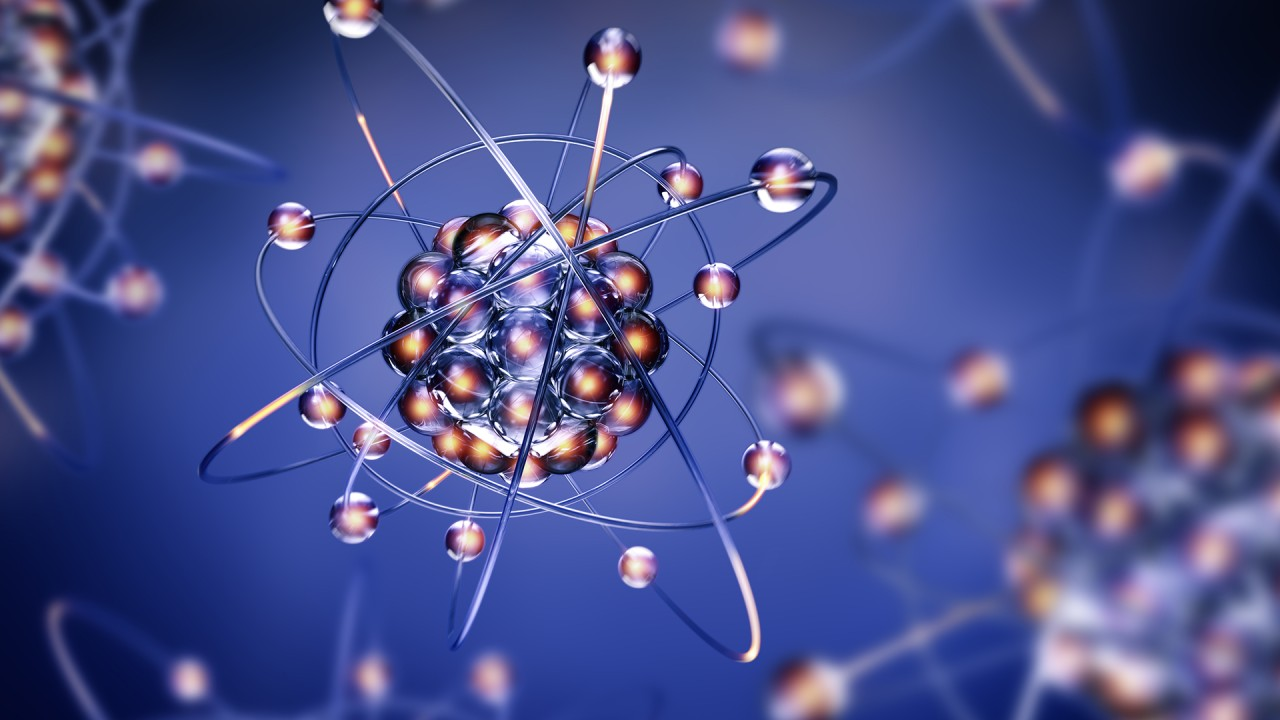
\includegraphics[width=\textwidth, height=0.9\textheight, keepaspectratio]{atom.jpg}
        \figciteweb{Bonn.19.08.2021}
        % \vspace{0.5cm}
        % \begin{quote}
        %     {Stellen Sie sich vor, das Universum ist ein riesiger Zoo, bevölkert mit einer unglaublichen Vielfalt an exotischen Lebewesen – den Teilchen. Einige sind uns vertraut, wie Elektronen oder Protonen, aber es gibt auch faszinierende, kurzlebige Kreaturen. Eine Gruppe davon sind die Hadronen, die ich euch heute Vorstellen möchte.}
        % \end{quote}
    \end{frame}

    % Title Slide
    \begin{frame}[noframenumbering, plain]
        \vspace*{-0.6cm}
        \titlepage
        \vspace*{-1.6cm}
    \end{frame}
    
    % Table of Contents
    \begin{frame}{Gliederung}
      \setcounter{page}{1}
        \tableofcontents
    \end{frame}
    
    \section{Einführung}
    \begin{frame}{Das Standardmodell der Elementarteilchen}
      \begin{figure}
        \centering
        \begin{minipage}{0.6\textwidth}
          \centering
          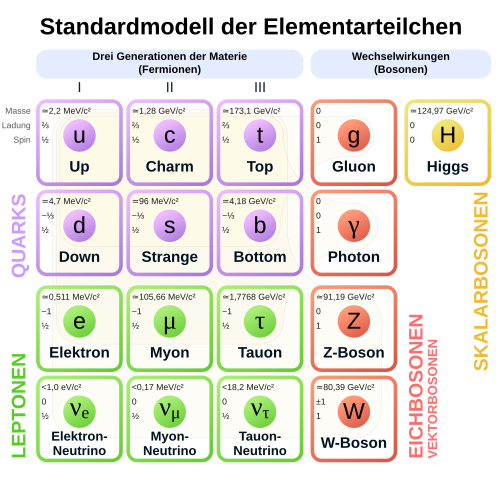
\includegraphics[width=\textwidth, keepaspectratio, height=0.9\textheight]{502px-Standard_Model_of_Elementary_Particles-de.svg.png}
        \end{minipage}
        \hfill
        \begin{minipage}{0.38\textwidth}
          \scriptsize
          \citeauthortitle[Von MissMJ \& Cush / abgeleitetes Werk: Polluks - Standard Model of Elementary Particles.svg, Gemeinfrei, \url{https://commons.wikimedia.org/w/index.php?curid=11307906} \\aus: ][]{Wikipedia.Standardmodell}
        \end{minipage}
      \end{figure}
    \end{frame}

    \begin{frame}{Hadronen: Aufbau und Klassifizierung}
      \begin{itemize}
        \item Baryonen (drei Quarks: Proton, Neutron, etc.)
        \item Mesonen (Quark-Antiquark-Paare, z.B. Pion, Kaon, etc.)
        \item Zusammengesetzt aus Quarks, die durch die starke Wechselwirkung gebunden sind
        \item Unterliegen den Quantenzahlen (Isospin, Strangeness, etc.)
      \end{itemize}
      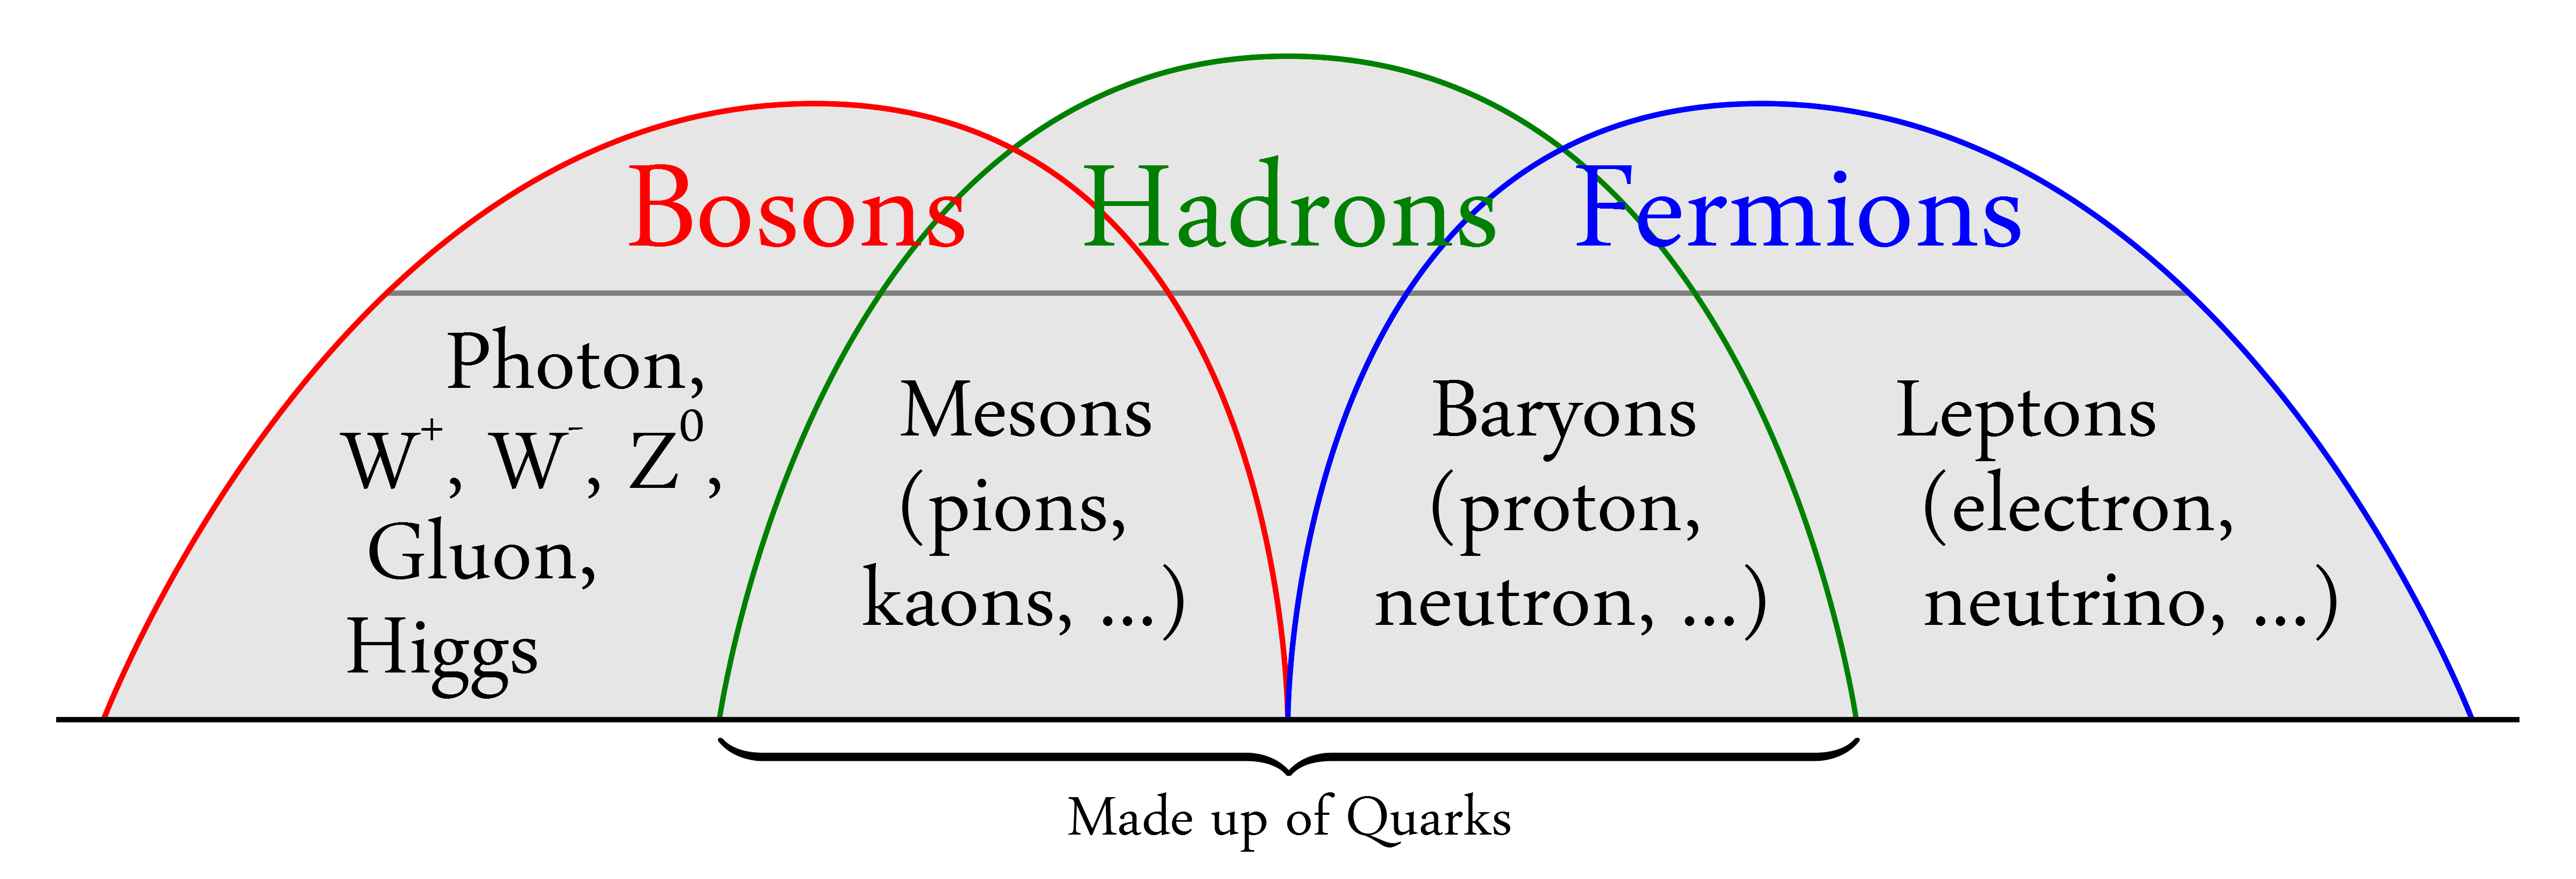
\includegraphics[width=\textwidth, height=0.4\textheight, keepaspectratio]{Bosons-Hadrons-Fermions-RGB-png2.png}
      \figciteweb{Wikipedia.Hadron}
    \end{frame}

    % \subsection{SU\(_3\) Dekuplett}
    \begin{frame}%{Das SU\(_3\) Dekuplett}
      \begin{figure}
        \centering
        \begin{minipage}{0.6\textwidth}
          \centering
          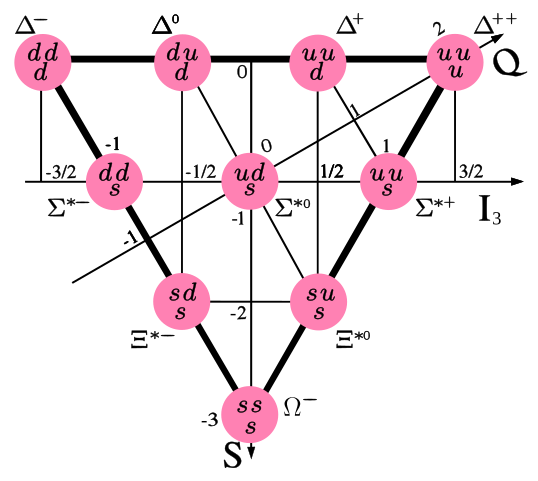
\includegraphics[width=\textwidth, keepaspectratio, height=0.9\textheight]{538px-Baryon-decuplet-small.svg.png}
        \end{minipage}
        \hfill
        \begin{minipage}{0.38\textwidth}
          \begin{itemize}
            \item $I_3$: Isospin
            \item $S$: Strangeness
            \item $Q$: Hyperladung
          \end{itemize}
          \vspace*{0,5cm}
          \normalsize{\textbf{{$\rightarrow$ Einführung der \emph{Farbladung}}}}\vspace*{1cm}
          
          \scriptsize % hier muss ich am Layout weiterarbeiten
          \citeauthortitle[Von Trassiorf - Eigenes Werk, Gemeinfrei, \url{https://commons.wikimedia.org/w/index.php?curid=3245752} \\aus: ][]{Wikipedia.DeltaBaryon} 
        \end{minipage}
      \end{figure} % hier ist was mit der Überschrift falsch!!
    \end{frame}
    
    
    
    \begin{frame}{Exotische Hadronen: Pentaquarks \& Co}
      \begin{itemize}
        \item Pentaquarks (fünf Quarks)
        \item Tetraquarks (vier Quarks)
        \item Neue Entdeckungen, z.B. LHCb-Resultate
      \end{itemize}
    \end{frame}
    
    \section{Aktuelle Forschung \& Anwendungen}
    \begin{frame}{Moderne Experimente \& offene Fragen}
      \begin{itemize}
        \item LHC-Experimente (ATLAS, CMS, LHCb)
        \item Stabilität von Protonen, Neutronen
        \item Bedeutung für Kosmologie und Teilchenphysik
      \end{itemize}
    \end{frame}
    
    \begin{frame}{Schluss \& Ausblick}
      \begin{itemize}
        \item Zusammenfassung der wichtigsten Punkte
        \item Ausblick auf weitere Forschungsrichtungen
      \end{itemize}
      
      \centering
      \alert{Vielen Dank für Ihre Aufmerksamkeit!}
    \end{frame}

    % Bibliography    
    \begin{frame}[allowframebreaks, noframenumbering, plain]{Literaturverzeichnis}
   \printbibliography%[nottype=unpublished]
    \end{frame}

    % Black slide
    \begin{frame}[plain, noframenumbering]
        \begin{tikzpicture}[remember picture, overlay]
            \fill[black] (current page.south west) rectangle (current page.north east);
        \end{tikzpicture}
        Test~\cite{Aaij.2015,Aaij.2019,C.Amsler.2017,GellMann.1964,Zweig.1964,Zweig.1964b}
    \end{frame}

\end{document}
